\section{Redux} 
\subsection{Overview}
Redux is a npm module which manage the entire state of the website from client-side. It consists of:
\begin{itemize}
	\item Actions;
	\item Reducers;
	\item Store.
\end{itemize}
When the website is built, a default state for the store is set (it is defined into the reducer JavaScript file).
\subsection{Unidirectional pattern} 
Basically some actions are mapped by \textit{container components} into specific \textit{presentational components} through them props with \textit{Connect(arg1, arg2)} method. When a presentational component request a \textit{dispatch()} of a specific action, a reducer will complete the request by changing the store and returning a new instance of the application state. Each time the store is changed, the \textit{Render()} method of displayed components is called.
\textit{Redux} is the name of the pattern implemented by React and Redux, it is an evolution of \textit{Flux} pattern, the difference is that Flux uses more than one store.\\
\begin{figure}[H]
	\centering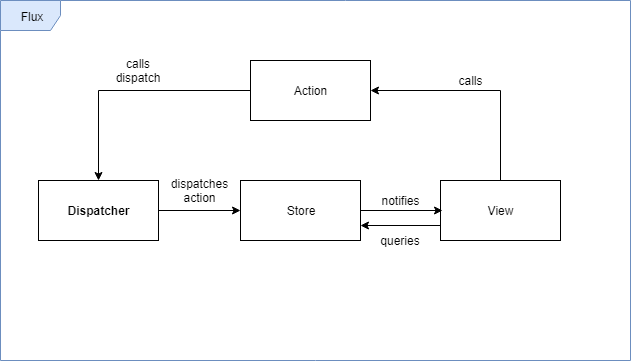
\includegraphics[scale = 0.6]{res/images/Flux.png}
	\caption{Flux pattern}
\end{figure}

\subsection{Actions}
There are twelve different actions inside \textit{src/actions/} folder. Each action is called by the \textit{action creator} when a container component request it's dispatch. Here there is the list of actions and what them do when they are invoked.
\begin{itemize}
	\item \textbf{ACLogin}: it changes the \texttt{logged} state value;
	\item \textbf{ACIncreaseQuantity}: it increases the quantity of a product that is inside the cart, by changing the \texttt{quantity} value of a specified product inside \texttt{cart} state value;
\end{itemize}
\subsection{Reducers}

\subsection{Store}

\subsection{Redux-Persist}
It is a npm module used for maintaining the current store even if the user leaves the website. It is browser-locally saved, so if a user will enter into the website from another device or from another browser, the store will be set with default values. It has a blacklist for bypassing some values, in this way reloading the website, these values will not be saved (the blacklist is defined into reducer JavaScript file).

\begin{landscape}
\subsection{UML} 

\begin{figure}[H]
	\centering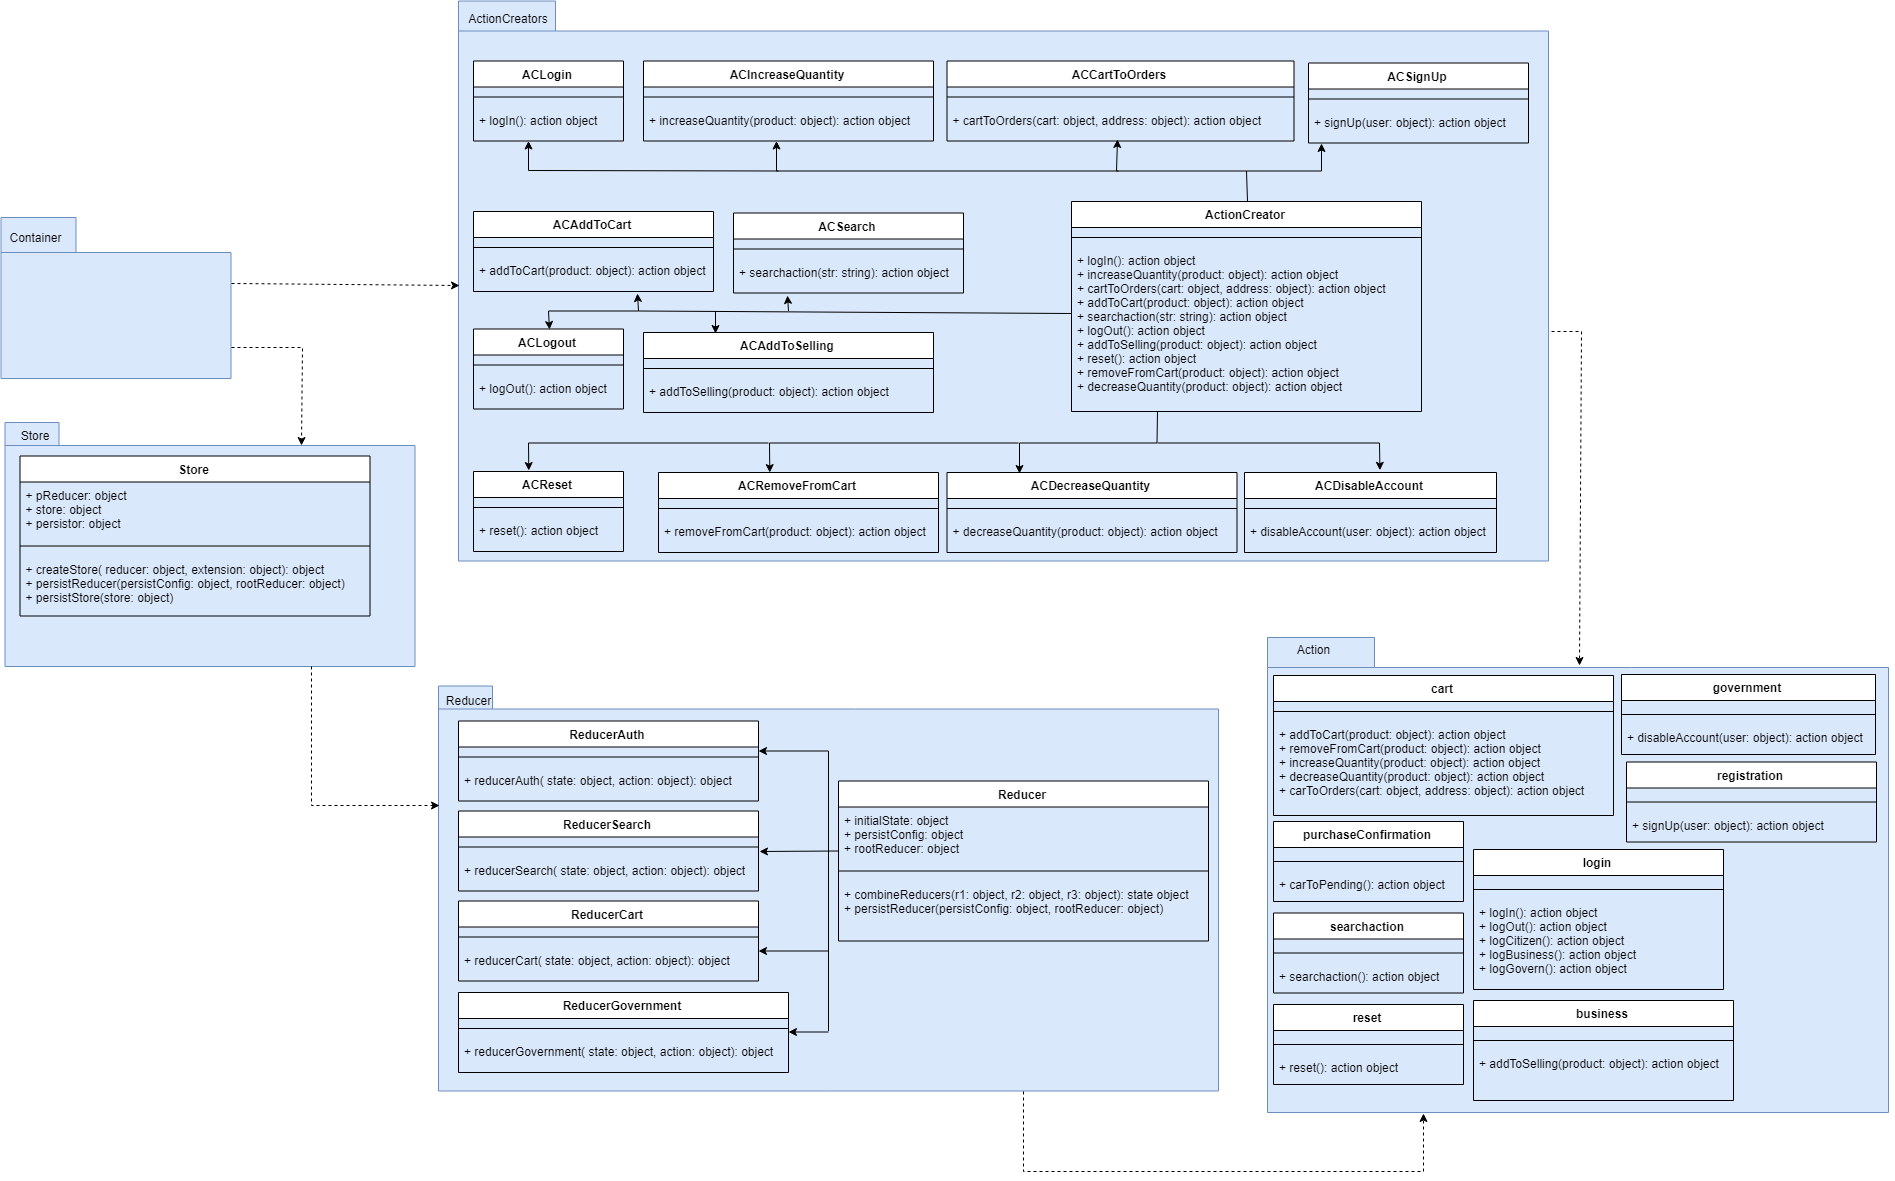
\includegraphics[scale = 0.3]{res/images/ReduxDiagram.png}
	\caption{Redux architecture}
\end{figure}
\end{landscape}